% Generated by calibration_section_20261030/make_calibration_section.py from the frozen
% calibration_pde_20261029 and calibration_positive_skew_20261031 outputs. No recalibration.
% AI-DRAFT blocks await the author's pass.
\subsection{Four-maturity calibrations on four option snapshots}
\label{sec:oca-calibration}
% [AI-DRAFT BEGIN: calibration data and conventions, rewritten point-first, 30 Oct 2026.]
We calibrate Heston and quadratic-drift LogSV jointly to four maturities of three
option surfaces observed on 15 July 2026: SPXW (weekly S\&P~500 index options), GLD
(options on the SPDR gold ETF) and TLT (options on the iShares 20+ year Treasury
bond ETF). The quotes are
ThetaData end-of-day option chains processed with the \texttt{option-chain-analytics}
package (OCA),\footnote{\url{https://github.com/ArturSepp/OptionChainAnalytics}. OCA
supplies the cached parity-implied forwards and discounts, the bid and ask implied
volatilities and the exact maturities used here. The report timestamps are
retained and are not synchronous closing executions.} which also supplies the
forward, discount and implied-volatility conventions. SPXW is the European
benchmark. GLD and TLT options are American, and for them OCA reports
European-equivalent Black implied volatilities, so the ETF examples compare smiles
under that convention and are not exact American-option prices. For each slice OCA
fits the European parity line $C-P=D(F-K)$ across strikes for the forward $F$ and
the discount $D$ and inverts the Black formula at these values, with no adjustment
for early exercise.
% [AUTHOR: the sentence above describes option-chain-analytics 6.0.2 (data/thetadata.py and
%  utils/forward_discount.py). Confirm that the cached surfaces were built with this routine.]
The ETF parity-implied
discounts exceed one in these slices and are normalisation inputs, not risk-free
curve estimates. Each surface uses the 27 July 2026 expiry (about 12 days) and
three further expiries: 14 August, 18 September and 16 October for SPXW and GLD
(about 30, 65 and 93 days), and 14, 21 and 28 August for TLT (about 30, 37 and 44
days). After the filters (positive ordered premiums, $|\log(K/F)|\leq0.15$, bid--ask
IV spread at most three volatility percentage points, at most 25 evenly spaced
strikes per slice plus the nearest ATM strike) the samples contain 103, 102 and 89
out-of-the-money quotes. All twelve slices have negative 25-delta smile skew, an
observable that is distinct from a fitted latent $\beta$.

A fourth snapshot, TLT on 2 August 2024 (denoted TLT+), exercises positive smile
skew with the same filters, objective, bounds and numerical checks. Its 99 quotes
span expiries 14 August, 30 August, 20 September and 30 September 2024 (about
12, 28, 49 and 59 days), and all four slices have positive 25-delta smile skew.
The candidate search tried GLD first, then TLT, requiring four usable maturities
and a positive 30-day skew, and the strict all-four-positive rule was not relaxed.
The selected snapshot maximises the 30-day skew among eligible TLT candidates.
The GLD archive holds 22 dates, all in July 2026, and no qualifying positive
30-day skew, whereas the TLT archive has 805 dates from June 2023 to August 2026, of which
196 have positive 30-day skew. This unequal coverage and the deliberate extreme
selection make TLT+ a methodological illustration, not an estimate of positive-skew
frequency across markets. The shorter expiry is retained in both models' joint fits.
% [AI-DRAFT END]

\paragraph{Objective and numerical implementation.}
The objective gives equal weight to each maturity and equal weight to retained
strikes within each maturity, and it targets the midpoint of bid and ask IVs.
For a parameter vector $\Theta$, $M=4$ maturities and $n_i$ retained strikes at maturity
$i$, define the decimal-IV residual
$e_{ij}(\Theta)=\sigma^{\mathrm{model}}_{ij}(\Theta)
-(\sigma^{\mathrm{bid}}_{ij}+\sigma^{\mathrm{ask}}_{ij})/2$. We minimise
\begin{equation}
 J(\Theta)=\frac{1}{M}\sum_{i=1}^{M}\frac{1}{n_i}\sum_{j=1}^{n_i}e_{ij}(\Theta)^2,
 \qquad \mathrm{RMSE}_{\mathrm{pp}}=100\sqrt{J(\Theta)}.
 \label{eq:oca-calibration-objective}
\end{equation}
Here $\mathrm{RMSE}_{\mathrm{pp}}$ is the root-mean-square error (RMSE) in volatility
percentage points (pp). Heston has five fitted parameters and LogSV six, and one
parameter vector fits all four maturities. We impose positive levels and drift
speeds and Heston $|\rho|<1$. For LogSV we fit the margin
$m=\kappa_2-\max(\beta,0)$ with $m\geq0.05$, which keeps $\kappa_2\geq0$ and
$\kappa_2\geq\beta$, the domain of Proposition~\ref{prop:martingale}, with a
numerical buffer. Heston's Feller condition is not imposed.

Heston uses its transform kernel, and every price is rechecked against a separately
coded characteristic function with adaptive quadrature. LogSV is calibrated with
the full-state backward transform PDE in log volatility, followed by Fourier
inversion, which retains the volatility-state dependence without truncating the
log transform to a finite polynomial.
Under the money-market measure, we use the
zero-carry normalisation $X_t=\log(S_t/S_0)$, so $X_0=0$.
For $y=\log\sigma$, $v^2=\beta^2+\varepsilon^2$ and
$U(t,y;\phi)=\E[\exp(-\phi X_t)\mid\sigma_0=e^y]$, the equation is
\begin{align}
 \partial_t U &= \tfrac12v^2\partial_{yy}U
   +\bigl[a(y)-\phi\beta e^y\bigr]\partial_yU
   +\tfrac12\phi(\phi+1)e^{2y}U, \qquad U(0,y;\phi)=1,
   \label{eq:oca-transform-pde}\\
 a(y)&=\kappa_1\theta e^{-y}+\kappa_2\theta-\kappa_1
       -\kappa_2e^y-\tfrac12v^2.\nonumber
\end{align}
Here $\Re\phi=-1/2$ is the valuation contour. The model is the Markovian specification
with a flat volatility backbone.
% [AI-DRAFT BEGIN: discretisation of the transform PDE, 17 Nov 2026, second pass. Taken from logvol_pde.py.]
The solver discretises $y$ on a uniform grid with spacing $\Delta y$, centred at
$\log\sigma_0$. It uses central differences, with the diffusion coefficient raised to
$\Delta y\,|a(y)|/2$ at nodes where that value exceeds $v^2/2$. The remote values are one at low volatility and zero at high
volatility. Two implicit Euler half steps precede the Crank--Nicolson steps and damp the
mismatch between the initial condition and the upper remote value.
% [AI-DRAFT END]

Two bounded coarse-grid optimisations use 401 state nodes and 256 time steps, one
started from a simulation-based fit and one from an independent starting
vector. The better solution is refined with 801 nodes and 512 steps. All optimiser
stages terminate successfully, which does not establish a global optimum. Reported
curves and scores use 1601 nodes and 1024 steps, with 64-point Gauss--Legendre
integration in each of six Fourier subintervals up to frequency 1600, on a
log-volatility domain of six units on either side of $\log\sigma_0$.

\begin{table}[htbp]\centering\small
\begin{tabular}{@{}l l r r r r@{}}\toprule
Market & Model & IV RMSE & 12-day RMSE & Inside spread & Fit time\\
 & & (pp) & (pp) & (\%) & (seconds)\\\midrule

SPXW & Heston & 0.698 & 1.127 & 8.7 & 0.16 \\

SPXW & LogSV (PDE) & 0.447 & 0.662 & 20.4 & 268.81 \\

GLD & Heston & 0.477 & 0.446 & 55.9 & 0.23 \\

GLD & LogSV (PDE) & 0.337 & 0.419 & 73.5 & 189.26 \\

TLT & Heston & 0.458 & 0.352 & 37.1 & 0.15 \\

TLT & LogSV (PDE) & 0.295 & 0.274 & 58.4 & 229.15 \\

TLT+ & Heston & 0.796 & 1.223 & 24.2 & 0.13 \\

TLT+ & LogSV (PDE) & 0.585 & 0.837 & 32.3 & 304.14 \\

\bottomrule\end{tabular}
\caption{LogSV lowers the in-sample IV RMSE on all four snapshots at one extra
parameter. Bounded fits to 103 SPXW, 102 GLD and 89 TLT quotes on 15 July 2026.
TLT+ denotes 99 quotes on 2 August 2024, not a second fit to the July TLT snapshot.
The total IV RMSE weights maturities equally, and the 12-day column reports the
shortest slice. Inside-spread percentages count quotes without weights. Heston
times are two-start transform calibrations run separately, and PDE times sum the two coarse
starts and the refinement, excluding simulation-based starting fits, just-in-time compilation warm-up
and validation. Source: ThetaData
via OCA.}
\label{tab:oca-fits}\end{table}

\begin{table}[htbp]\centering\small
\begin{tabular}{@{}l l r r r r r r r r@{}}\toprule
Market & Model & \multicolumn{4}{c}{IV RMSE (pp)} & \multicolumn{4}{c}{Inside spread (\%)}\\
\cmidrule(lr){3-6}\cmidrule(lr){7-10}
 & & 1 & 2 & 3 & 4 & 1 & 2 & 3 & 4\\\midrule

SPXW & Heston & 1.127 & 0.618 & 0.242 & 0.491 & 15 & 4 & 12 & 4 \\

SPXW & LogSV & 0.662 & 0.463 & 0.137 & 0.357 & 15 & 16 & 42 & 8 \\

GLD & Heston & 0.446 & 0.646 & 0.263 & 0.473 & 84 & 27 & 88 & 24 \\

GLD & LogSV & 0.419 & 0.359 & 0.266 & 0.278 & 88 & 69 & 77 & 60 \\

TLT & Heston & 0.352 & 0.515 & 0.445 & 0.503 & 65 & 38 & 33 & 20 \\

TLT & LogSV & 0.274 & 0.334 & 0.272 & 0.295 & 82 & 54 & 57 & 48 \\

TLT+ & Heston & 1.223 & 0.855 & 0.432 & 0.346 & 21 & 16 & 32 & 28 \\

TLT+ & LogSV & 0.837 & 0.682 & 0.355 & 0.277 & 25 & 16 & 48 & 40 \\

\bottomrule\end{tabular}
\caption{LogSV improves 15 of the 16 maturity slices, with the
largest gain at the 12-day SPXW slice. Maturities are numbered from the shortest:
about 12, 30, 65 and 93 days for SPXW and GLD and about 12, 30, 37 and 44 days for
TLT, and about 12, 28, 49 and 59 days for TLT+. Quote counts per slice are 17 to 26.
Source: ThetaData via OCA, with dates as in Table~\ref{tab:oca-fits}.}
\label{tab:oca-maturity}\end{table}

\begin{figure}[tbp]\centering
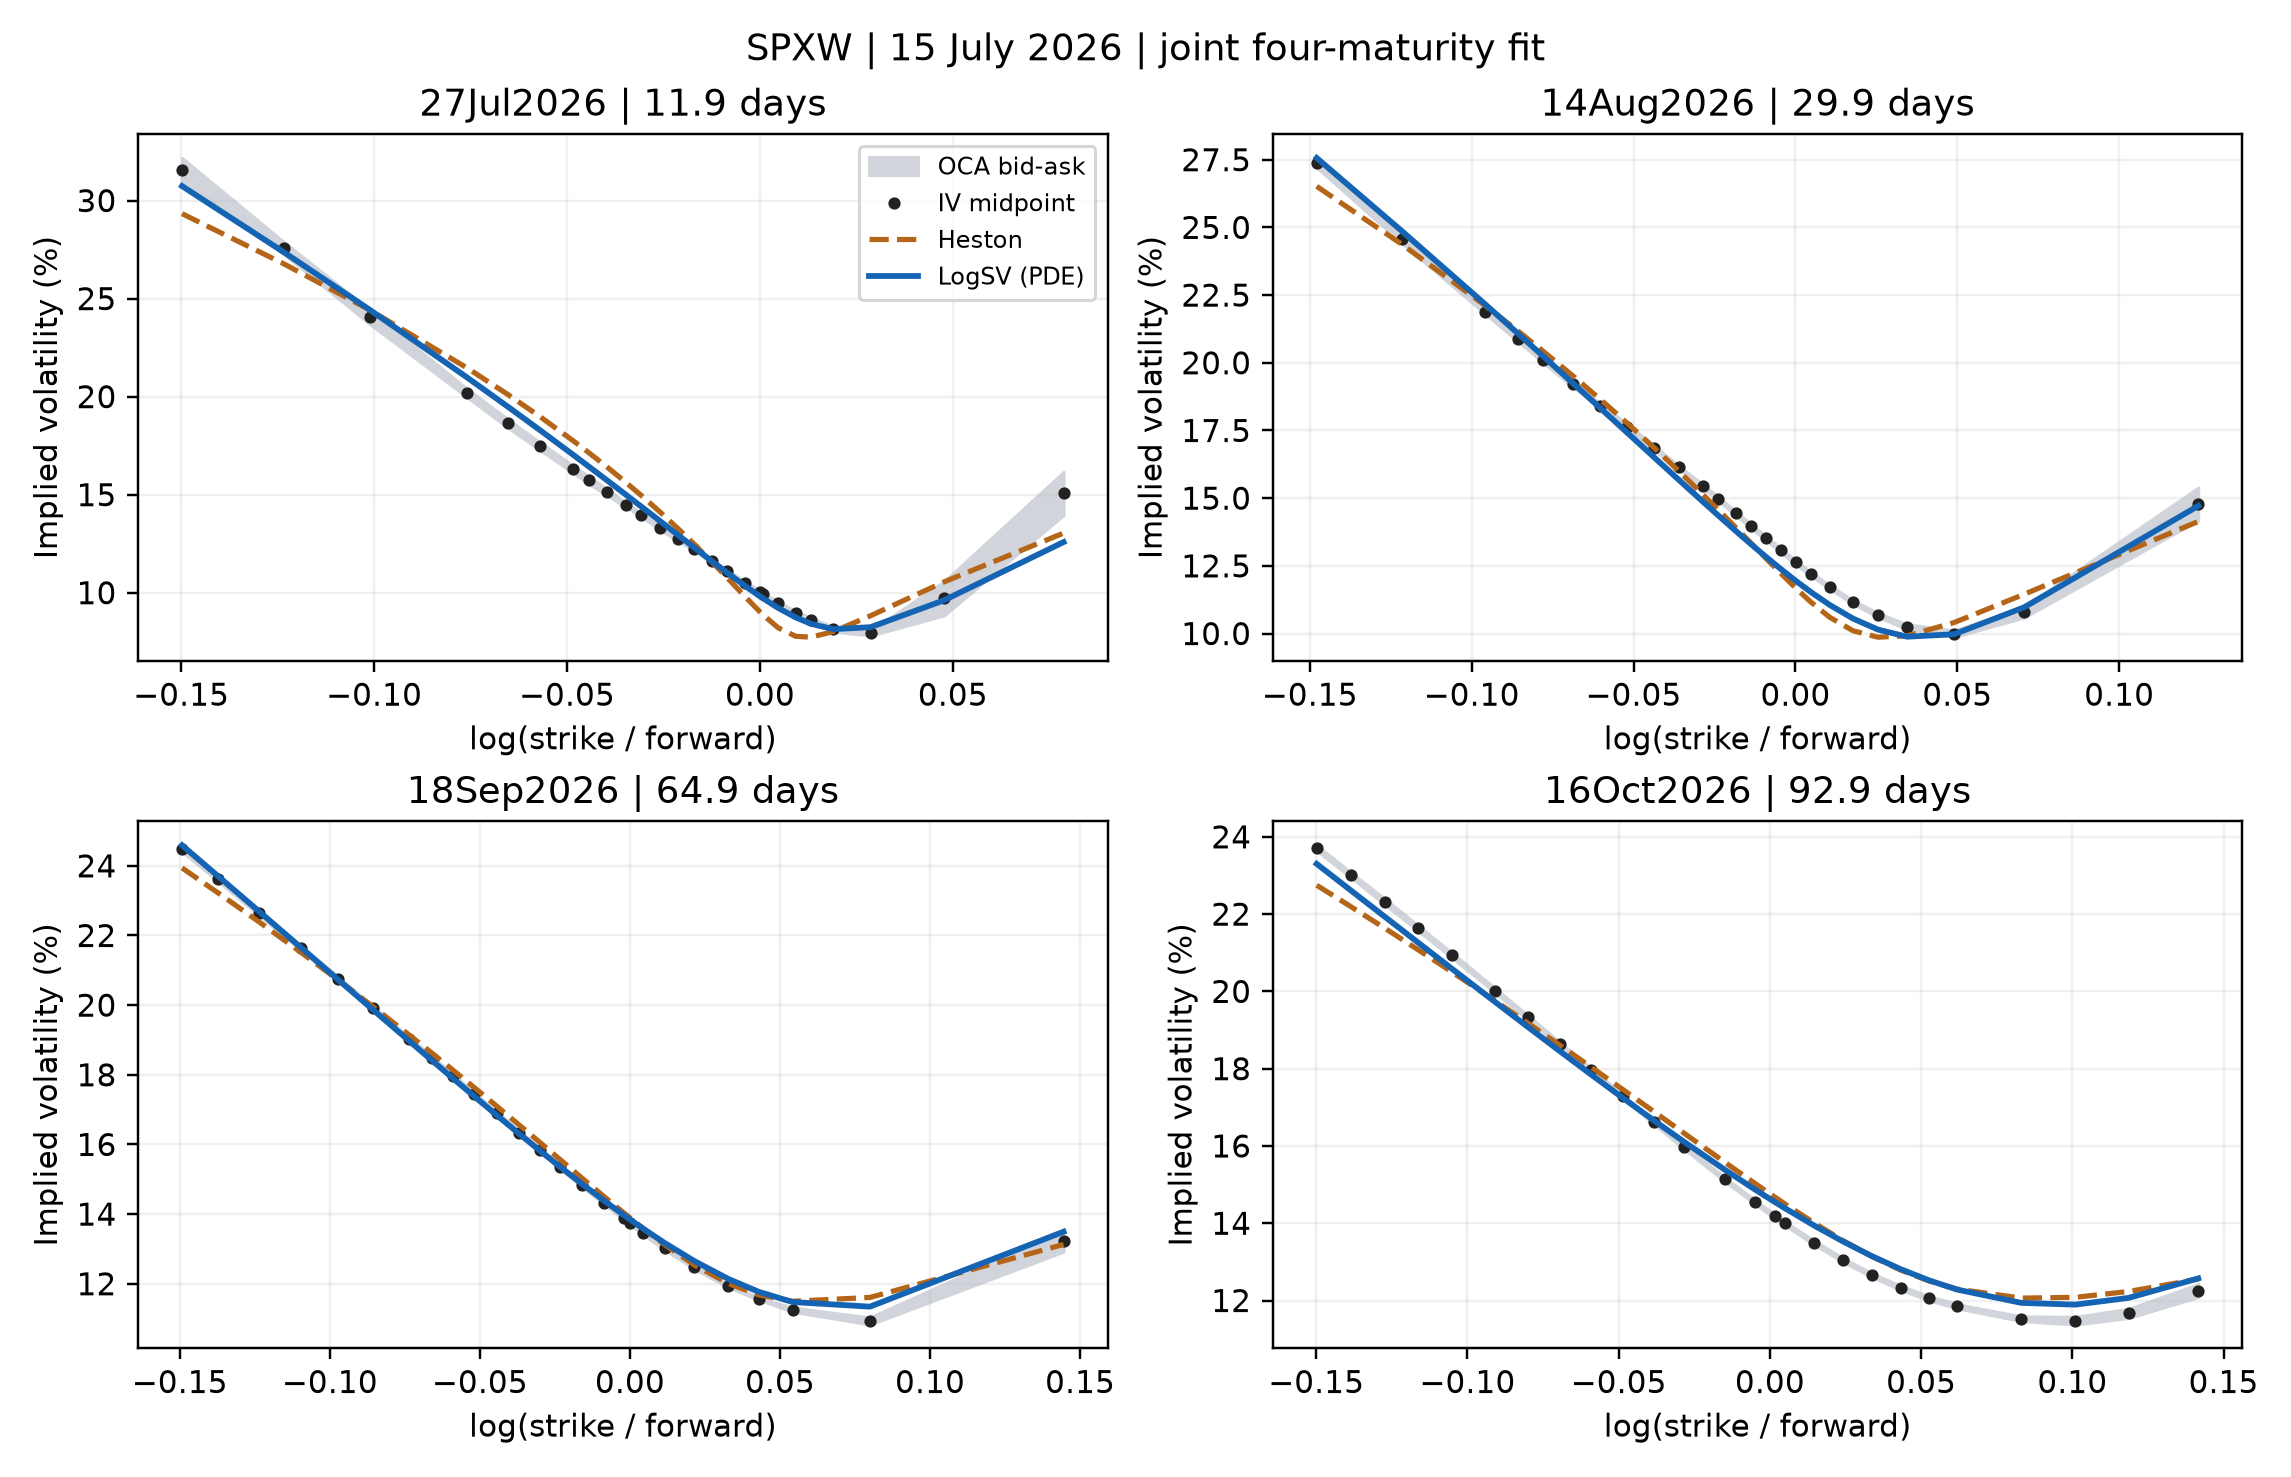
\includegraphics[width=\textwidth]{figures/calibration_pde_20261029/spxw_fits.png}
\caption{SPXW on 15 July 2026, including the approximately 12-day expiry. Points and grey bands show OCA midpoint and bid--ask IVs. The dashed curve is Heston and the solid curve the LogSV fit priced on the fine PDE grid. All four maturities share one parameter vector per model. Source: ThetaData via OCA.}\label{fig:oca-spxw}\end{figure}

\begin{figure}[tbp]\centering
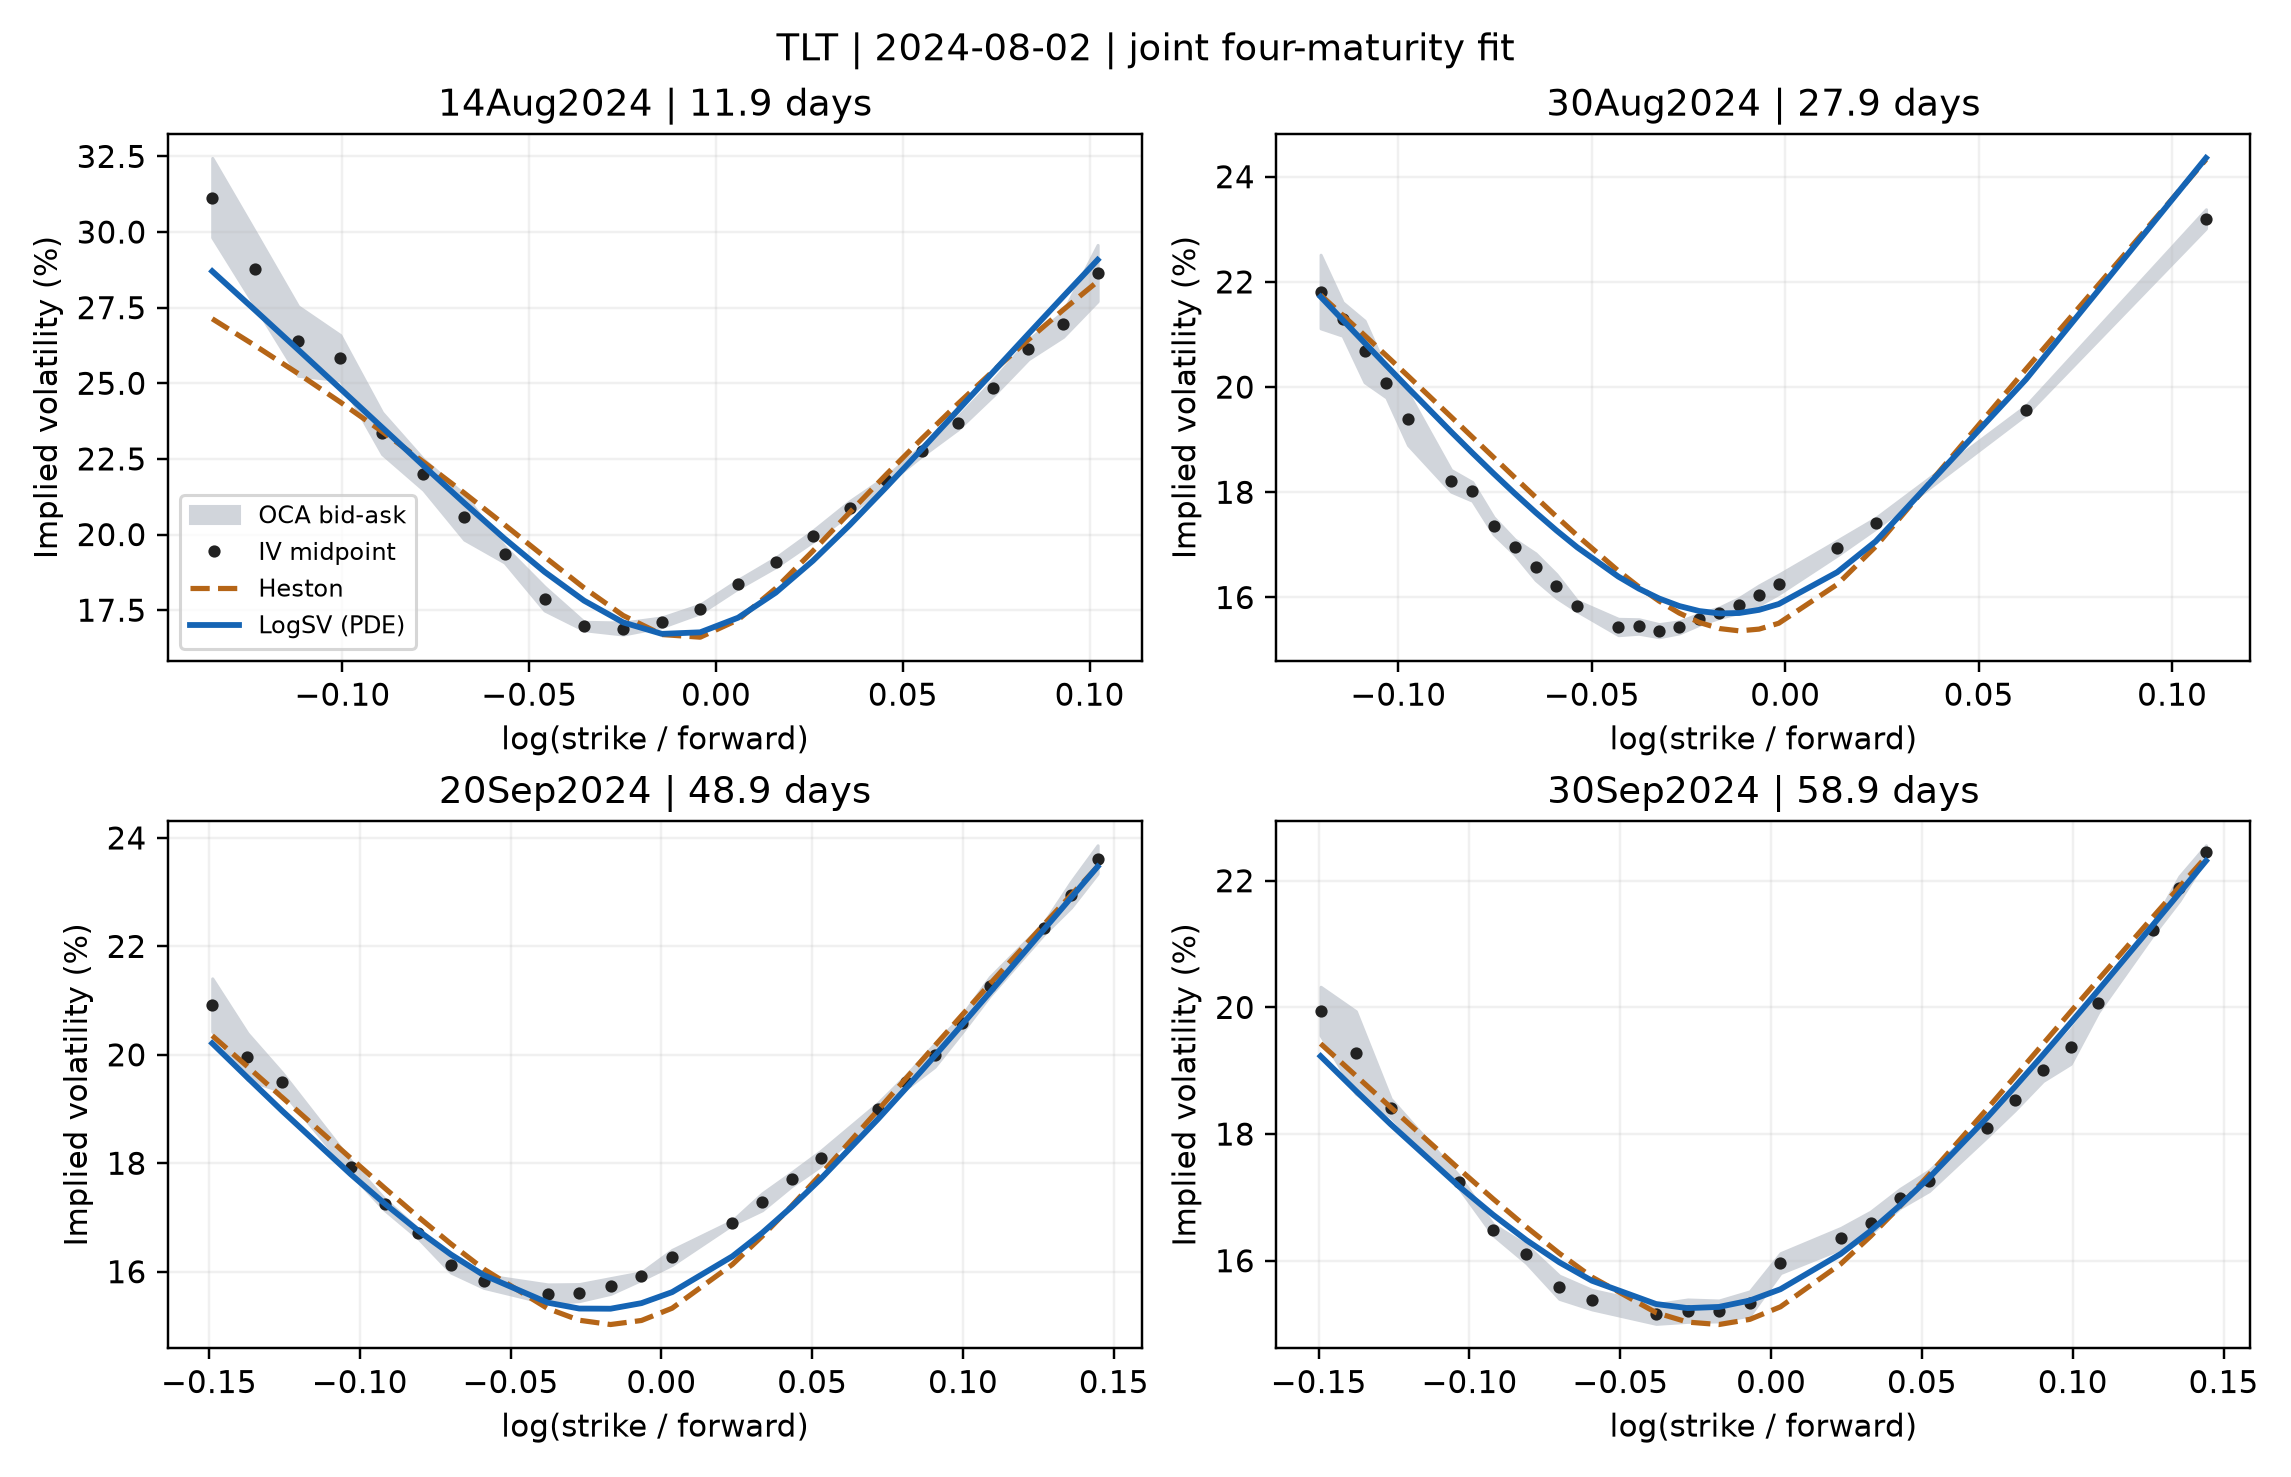
\includegraphics[width=\textwidth]{figures/calibration_positive_skew_20261031/tlt_fits.png}
\caption{TLT+ on 2 August 2024, including the approximately 12-day expiry. Points and grey bands show OCA midpoint and bid--ask IVs. The dashed curve is Heston and the solid curve the LogSV fit priced on the fine PDE grid. All four maturities share one parameter vector per model. The ETF panels use OCA European-equivalent Black IV conventions. Source: ThetaData via OCA.}\label{fig:oca-tltpositive}\end{figure}

% [AI-DRAFT BEGIN: per-maturity reading, information criterion and half-lives, 30 Oct 2026.]
Table~\ref{tab:oca-fits} summarises the four joint fits, and
Figures~\ref{fig:oca-spxw} and~\ref{fig:oca-tltpositive} show the SPXW and TLT+
smiles with both fitted curves. The GLD and July TLT smile figures are in the
replication package. Table~\ref{tab:oca-maturity} locates the improvement. On SPXW the LogSV RMSE at
the 12-day and 30-day slices is 0.66 and 0.46 percentage points against 1.13 and 0.62 for Heston, while the two longest slices differ by less. On GLD and TLT
the improvement is spread across maturities, and LogSV improves 15 of the 16 slices in total. A criterion of the Bayesian-information type
uses the unweighted per-quote sum $\mathrm{RSS}=\sum_{i,j}(100e_{ij})^2$,
evaluated at each model's fitted parameters, and $n=\sum_i n_i$, rather than the maturity-weighted objective in
\eqref{eq:oca-calibration-objective}. The statistic $n\ln(\mathrm{RSS}/n)+k\ln n$,
with $k=5$ for Heston and $k=6$ for LogSV, favours LogSV by SPXW: -88, GLD: -67, TLT: -76, TLT+: -56 (differences LogSV minus Heston, so negative values favour LogSV). The quotes
within a slice are not independent and some fitted parameters are at their bounds,
so the criterion is descriptive and the penalty
for the sixth parameter, $\ln n\approx4.6$, is small against the residual term.
The fitted parameters in Tables~\ref{tab:oca-logsv-params}
and~\ref{tab:oca-heston-params} carry linearised drift half-lives
$365\ln2/(\kappa_1+\kappa_2\theta)$ of 7.4 to 10.0 days for LogSV
and variance-mean half-lives $365\ln2/\kappa$ of 8.4 to 10.4 days for Heston, with active upper bounds on the drift speeds in
every LogSV fit and in the GLD and TLT+ Heston fits. Both models use their mean reversion to
shape the 12-day slice. The drift parameters are therefore term-structure parameters
of one snapshot, not estimates of historical mean reversion. The LogSV half-life
describes the drift linearised at $\theta$, rather than the exact conditional mean
or stationary autocorrelation. Heston's expression is exact for its conditional
variance mean.
% [AI-DRAFT END]

\begin{table}[htbp]\centering\small
\begin{tabular}{@{}l r r r r r r r r@{}}\toprule
Market & $\sigma_0$ & $\theta$ & $\kappa_1$ & $\kappa_2$ & $\beta$ & $\varepsilon$ & $\kappa_2-\beta$ & Half-life (days)\\\midrule

SPXW & 0.0722 & 0.1359 & 30.0000 & 1.5350 & -4.1765 & 4.7239 & 5.7115 & 8.4 \\

GLD & 0.1808 & 0.3021 & 1.2073 & 80.0000 & -1.2408 & 4.3198 & 81.2408 & 10.0 \\

TLT & 0.0758 & 0.0777 & 30.0000 & 13.6871 & -0.7883 & 5.7683 & 14.4754 & 8.1 \\

TLT+ & 0.1813 & 0.1280 & 30.0000 & 31.0183 & 1.4335 & 6.8799 & 29.5848 & 7.4 \\

\bottomrule\end{tabular}
\caption{PDE-calibrated LogSV parameters. The three July snapshots have $\beta<0$, and
TLT+ has $\beta>0$ and satisfies $\kappa_2>\beta$ with a wide margin. The imposed
lower bound $m=0.05$ is inactive for TLT+. Active bounds: SPXW $\kappa_1=30$, GLD $\kappa_2=80$, TLT $\kappa_1=30$, TLT+ $\kappa_1=30$. The linearised drift half-life is
$365\ln2/(\kappa_1+\kappa_2\theta)$. Source: ThetaData via OCA, with dates as in Table~\ref{tab:oca-fits}.}
\label{tab:oca-logsv-params}\end{table}

\begin{table}[htbp]\centering\small
\begin{tabular}{@{}l r r r r r r@{}}\toprule
Market & $V_0$ & $\theta_V$ & $\kappa$ & $\rho$ & $\nu$ & Half-life (days)\\\midrule

SPXW & 0.00353 & 0.03453 & 24.26049 & -0.64219 & 2.79164 & 10.4 \\

GLD & 0.04286 & 0.06558 & 30.00000 & -0.27978 & 2.77467 & 8.4 \\

TLT & 0.00585 & 0.01156 & 26.68251 & -0.13692 & 1.71334 & 9.5 \\

TLT+ & 0.04433 & 0.02625 & 30.00000 & 0.19569 & 3.11254 & 8.4 \\

\bottomrule\end{tabular}
\caption{Heston variance parameters. GLD and TLT+ reach the $\kappa=30$ upper bound. All
four solutions have $2\kappa\theta_V<\nu^2$, and the transform pricer accommodates
the attainable, instantaneously reflecting zero variance boundary of the usual CIR
solution. The conditional variance-mean half-life is $365\ln2/\kappa$. Source: ThetaData via OCA, with dates as in Table~\ref{tab:oca-fits}.}
\label{tab:oca-heston-params}\end{table}

\paragraph{Numerical checks.}
We separately double the spatial and the time resolution, enlarge the state domain
from six to eight log-volatility units at matched mesh spacing, and refine the
Fourier integration to 96 points per subinterval and cutoff 2400. Table~\ref{tab:oca-pde-checks}
reports the largest changes relative to the reported grid, in IV units and relative
to each quote's premium bid--ask spread, including the worst quote.

\begin{table}[htbp]\centering\small
\begin{tabular}{@{}l r r r r@{}}\toprule
Market & Grid IV change & Grid/spread & PDE--MC gap & MC steps\\
 & (pp, max.) & (\%, max.) & (bp of $F$, max.) & \\\midrule

SPXW & 0.00074 & 0.150 & 0.0187 & 512 \\

GLD & 0.00005 & 0.003 & 0.0067 & 1024 \\

TLT & 0.00014 & 0.021 & 0.0027 & 512 \\

TLT+ & 0.00027 & 0.057 & 0.0135 & 512 \\

\bottomrule\end{tabular}
\caption{All observed deterministic refinement changes are below one percent of a
premium spread at every retained quote, and independent Monte Carlo (MC) comparisons are
reported alongside them. Checks use the final PDE-calibrated parameters. Grid
columns take the maximum over four separate refinements. MC uses four independent
scrambles of 32768 paths each with paired half-step comparisons. Price differences
are discounted premiums divided by the forward, times $10^4$.}
\label{tab:oca-pde-checks}\end{table}

The largest deterministic refinement change is 0.00074 IV percentage
points and 0.150\% of a premium spread. Independent conditional
split-step Monte Carlo gives a maximum standardised price gap of 3.50, and 6 of the 393 quotes lie outside two
estimated scramble standard errors. Four scrambles give noisy standard-error
estimates, so these are not simultaneous tests. The simulator reports no volatility
flooring, and the Heston independent-pricing checks are retained in the replication package.

\paragraph{Cost, accuracy and what the examples support.}
% [AI-DRAFT BEGIN: speed and expansion status stated directly (E4), 30 Oct 2026.]
The PDE calibration costs 806 to 2,367 times the Heston transform calibration on these surfaces
(Table~\ref{tab:oca-fits}). These ratios compare the two implementations and their
starting protocols and do not isolate an intrinsic model cost. PDE fits include
two coarse starts and refinement, while simulation-based starting fits and validation
are excluded. A state-dependent PDE is solved at each Fourier frequency.
The second-order affine expansion of \citet{SeppRakhmonovLogSV} closes most of that
gap when it is accurate, but in the package's pricing diagnostics its truncation error is of
the same order as the smile residuals, and tighter solver tolerances, subdivision,
recentring and higher polynomial degree do not provide a general cure. We therefore
use the PDE for the objective and the displayed prices, reserve the expansion for
parameter regimes in which it has been validated against the PDE, and record the
regime boundary as an open implementation item.

The examples support limited conclusions. LogSV lowers the midpoint IV
RMSE on all four snapshots at one extra parameter, on 15 of 16 maturity
slices, with the largest gain at the 12-day SPXW slice. A numerically validated pricer does not make the model
fit each bid--ask interval, and the SPXW smile residuals remain material. The
implementation sequence that produced these numbers, a deterministic coarse-grid
fit, finer-grid refinement and independent checks at the final parameters judged
against market spreads, is the reusable part. The examples do not rank the model
families across assets and do not estimate historical mean reversion.

The TLT+ fit gives $\beta=\positiveBeta$ and $\kappa_2=\positiveKappaTwo$, hence
$\kappa_2-\beta=\positiveMargin$, and Heston gives $\rho=\positiveHestonRho$.
Its IV RMSE falls from \rmseHestonTLTpositive\ to \rmseLogSVTLTpositive\ percentage
points and its inside-spread share rises from \insideHestonTLTpositive\% to
\insideLogSVTLTpositive\%. The positive-dependence fit is admissible, with a slack
imposed constraint, and does not exercise $C=\beta$. Neither fitted coefficient is
the historical index beta of Section~\ref{sec:empirical-beta}. The ETF quotation
qualification applies.
% [AI-DRAFT END]

